\documentclass{article}
\usepackage[utf8]{inputenc}

\title{Report.1.OpenMP.tex}
\author{gw.muraro }
\date{29 October 2018}

\usepackage{natbib}
\usepackage{graphicx}
\usepackage{pgfplots}

\begin{document}

\maketitle

\section{Usage of OpenMP} \newline
\begin{itemize}
    \item How you implement the conversion ? \newline
    I pasted the same code and added the following OpenMP directive in order to split the for loop : 
    \begin{verbatim}
        #pragma omp parallel for 
        for (...){...}
    \end{verbatim}
    I also add a new method which parallelize the two for loops. It is called /**/
        
    \item What’s the speedup? \newline
        On the ICT 3 machine, we got these results :
        \newline
    \begin{verbatim}
        USTH ICT Master 2018, Advanced Programming for HPC.
        Warming up...
        Starting labwork 1
        labwork 1 CPU ellapsed 3662.1ms
        labwork with double pragma ellapsed 790.9ms
        labwork 1 ellapsed 873.6ms
    \end{verbatim}
        
    We can see that we reduce by 4 the calculation time, and we gain around 100ms by parallelizing the second for loop, reducing now by 5 the initial computing time. 
    
    \item Try experimenting with different OpenMP parameters \newline
    %%plot
    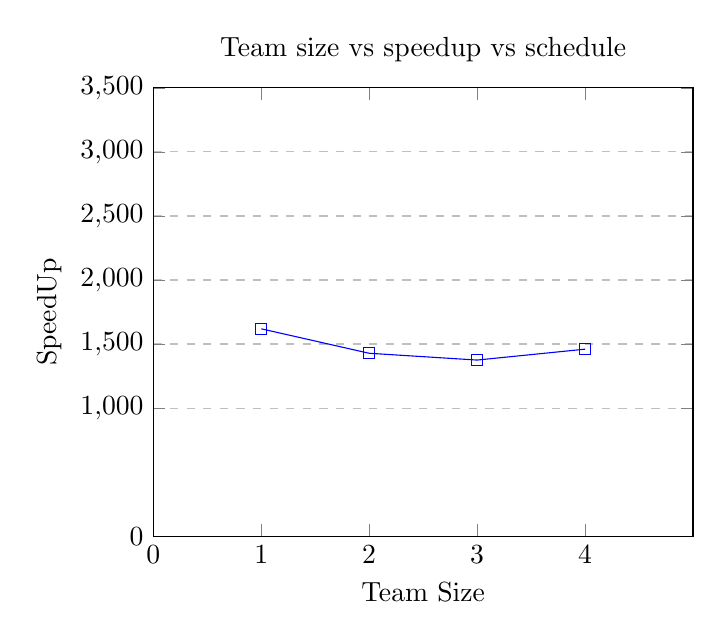
\begin{tikzpicture}
        %%define axes
        \begin{axis}[
            title={Team size vs speedup vs schedule},
            xlabel={Team Size},
            ylabel={SpeedUp},
            xmin=0, xmax=5,
            ymin=0, ymax=3500,
            xtick={0,1,2,3,4},
            ytick={0,1000,1500,2000,2500,3000,3500},
            legend pos=north west,
            ymajorgrids=true,
            grid style=dashed,
        ]
        %% data filing
        \addplot[
            color=blue,
            mark=square,
            ]
            coordinates {
            (1,1619)(2,1428)(3,1375)(4,1460)
            };

        \end{axis}
    \end{tikzpicture}
\end{itemize}

\end{document}

